\section{Experiments}
\label{sec:experiments}
In this section, we evaluate our method using  TU-Berlin sketch benchmark. It contains 250 classes. Each class has 80 instances. We do a group of experiments to compare our method with other methods in recognition accuracy and trainable parameters. Like previous works, we use 3-fold cross-validation within the dataset.  We use sketch dataset augmentation scenario  ~\cite{Yu2015SketchaNetTB} to ease our over-fitting problem(see Fig ~\ref{fig:aug_data}).

\begin{figure}[htbp]
    \center
    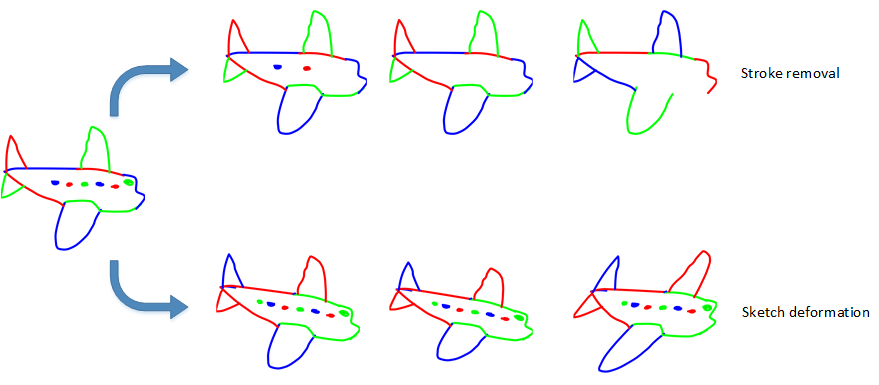
\includegraphics[width=3in]{images/aug_data.png}
    \fcaption{Sketch data augmentation.}
    \label{fig:aug_data}
\end{figure}

\subsection{Recognition accuracy with different $N$}
\label{ssec:resample_number}

From the Fig.~\ref{fig:resample}, we can see that 256 points are enough to represent the airplane. But in TU-Berlin dataset, there are many instances with lots of strokes that 256 points are not enough to represent an examples. In order find a proper $N$, we did a group experiments with $N = 1024, 512, 256, 128$. If $N$ is too large, there are no good for recognition accuracy, but makes the model slower.

\begin{table}[htbp]
\begin{tabular}{|p{1.4cm}|p{1.3cm}|p{1.3cm}|p{1.3cm}|p{1.3cm}|}
    \hline
     $N$ & 1024& 512 & 256 & 128\\
    \hline
     Accuracy & x\% & x\% & x\%& x\%\\
    \hline
\end{tabular}
\caption{Recognition with different $N$.}
\end{table}

\subsection{Training strategy}
\label{ssec:training_strategy}
When we train PointNet ~\cite{qi2017pointnet} model for sketch recognition. The recognition accuracy on training dataset is extremely high and lower over than 20\% on evaluation dataset. It shows that PointNet is easy to overfit. SketchPointNet is a multi-stage PointNet. It also suffers from overfitting problem. In order to ease overfitting problem, we design a training strategy for SketchPointNet: (i) we random initialize all the parameters in the SketchPointNet for the first time of training ; (ii) after the latest round of training, we initialize parameters in P1 and P2 with last trained parameters and random initialize parameters in P3, then, we retrain the SketchPointNet; (iii) keep doing the last step till the recognition accuracy on evaluation dataset is stable.

From the Table ~\ref{tbl:iteration}, we can see that the recognition results on evaluation dataset are getting higher and higher after numbers of iterations of training. It shows that our training strategy is effective. The training parameters are densely distributed in P3. P3 is more tend to converge on training dataset without sufficient training for P1 and P2. So we reinitialize parameters randomly in P3 to ensure that the parameters in P1 and P2 are keeping updated. 

\begin{table}[htbp]
\centering
\begin{tabular}{llll}
    \hline
     Iteration& 1&  2& 3\\
    \hline
     split 1& 70.8 \% & 73.8\% & 74.3\% \\
     split 2& 71.2\% & 73.6\% & 74.3\% \\
     split 3& 70.8\% & 72.5\% & 74.0\% \\
    \hline
\end{tabular}
\caption{Training results with multi-iterations on 3 folders.}
\label{tbl:iteration}
\end{table}

\subsection{Comparison of different methods in number of parameters and recognition accuracy}
\label{ssec:cm_speed}
SketchPointNet is derived from PointNet. It uses lots of shared architecture, which means less parameters compared with existing Image-based sketch recognition approaches. We performed Sketch-a-Net(vallina) ~\cite{Yu2015SketchaNetTB}, DeepSketch 1 ~\cite{Seddati2015DeepSketchDC} and SketchPointNet on Titan 1080 with tensorflow 1.2. The whole model of Sketch-a-Net ~\cite{Yu2015SketchaNetTB} and DeepSketch 2 \cite{Dupont2016DeepSketch2D} use different feature fusion method, which makes the whole models too large. So we only compare 3 end-to-end networks(Sketch-a-Net(vallina), DeepSketch 1 and SketchPointNet).

\begin{table}[htbp]
\centering
\begin{tabular}{lll}
    \hline
     Models& Trainable Parameters&  Storage\\
    \hline
     Sketch-a-Net(vallina) ~\cite{Yu2015SketchaNetTB}&8.24 million& 64M\\
     DeepSketch 1 ~\cite{Seddati2015DeepSketchDC}& 55.1 million& 223M\\
     Ours&\textbf{0.94} million& \textbf{20}M\\
    \hline
\end{tabular}
\caption{Comparison of trainable parameters.}
\label{tbl:model_size}
\end{table}

\begin{table*}
\centering
\small
\begin{tabular}{lllll}
    \hline
     models&group parameters& time/sketch& accuracy &memory\\
    \hline
     SketchPointNet1(mlp(8,16,64), mlp(32,32,128), mlp(64,128,1024))&group1(512*30), group2(256*100)& 163.8ms& 73.5\% & 3.11G\\
    \hline
     Sketch-a-Net& - &82.7ms& 77.9\% & 529M\\
    \hline
     DeepSketch 1& - &106.3ms& 75.42\% & 573M\\
    \hline
\end{tabular}
\caption{Performance comparison of different networks(cpu).}
\label{tbl:speed_cpu}
\end{table*}

\begin{table*}
\centering
\begin{tabular}{llll}
    \hline
     models&group parameters& accuracy& stroke order\\
    \hline
     SketchPointNet(mlp(8,16,64), mlp(32,32,128), mlp(64,128,1024))&group1(512*30), group2(256*100)& 73.5\% & y\\
    \hline
     SketchPointNet(mlp(8,16,64), mlp(32,32,128), mlp(64,128,1024))&group1(512*30), group2(256*100)& 69.6\% & n\\
    \hline
     PointNet++(mlp(8,16,64), mlp(32,32,128), mlp(64,128,1024))&group1(512*30), group2(256*100)& 51.2\% &n\\
    \hline
     PointNet++(mlp(64,64,128), mlp(128,128,256), mlp(256,512,1024))&group1(512*64), group2(128*64)& 58.7\% &n\\
    \hline
     PointNet(mlp(64,64,64,128,1024))&-& 46\% &n\\
    \hline
\end{tabular}
\caption{Comparing with PointNet and PointNet++}
\label{tbl:pointnet_cp}
\end{table*}

From the tabel ~\ref{tbl:model_size} we can see that our model need fewer trainable parameters than Sketch-a-Net(vallina) and DeepSketch 1. Although our model are smaller compared with existing DNN-based appraches. We still achieve a high recognition accuracy.

\begin{table}[htbp]
\centering
\large
\begin{tabular}{ll}
    \hline
     Models &Accuracy\\
    \hline
     HOG-SVM ~\cite{Eitz2012HowDH}& 56\% \\
     MKL-SVM ~\cite{LiHSG15} & 65.8\% \\
     FV-SP ~\cite{Schneider2014SketchCA} & 68.9\% \\
     LeNet ~\cite{LeCun1998GradientbasedLA}& 55.2\% \\
     Sketch-a-Net(vallina) ~\cite{Yu2015SketchaNetTB}& 72.6\% \\
     Sketch-a-Net ~\cite{Yu2015SketchaNetTB}& \textbf{77.95}\% \\
     DeepSketch 1 ~\cite{Seddati2015DeepSketchDC}& 75.42\% \\
     DeepSketch 2 ~\cite{Dupont2016DeepSketch2D}& 77.69\% \\
     \hline
     PointNet++ ~\cite{qi2017pointnetplusplus}& 66.53\% \\
     PointCNN ~\cite{1801.07791}& 67.72\% \\
     Ours& 74.2\% \\
    \hline
\end{tabular}
\caption{Sketch recognition with different models.}
\label{tbl:acc}
\end{table}

\begin{table}[htbp]
\centering
\large
\begin{tabular}{ll}
    \hline
     Models &Accuracy(@5)\\
    \hline
     DeepSketch 2 ~\cite{Seddati2015DeepSketchDC}& 94.52\% \\
     Ours& 92.3\% \\
    \hline
\end{tabular}
\caption{Top-5 sketch recognition accuracy.}
\label{tbl:acc}
\end{table}

Fig. ~\ref{fig:resshow} shows some results. Although our network can handle some challenging cases(green). SketchPointNet still fail on very ambiguous cases(the reds are predictions, the blacks are ground truth for each case).

\begin{figure}[htbp]
    \center
    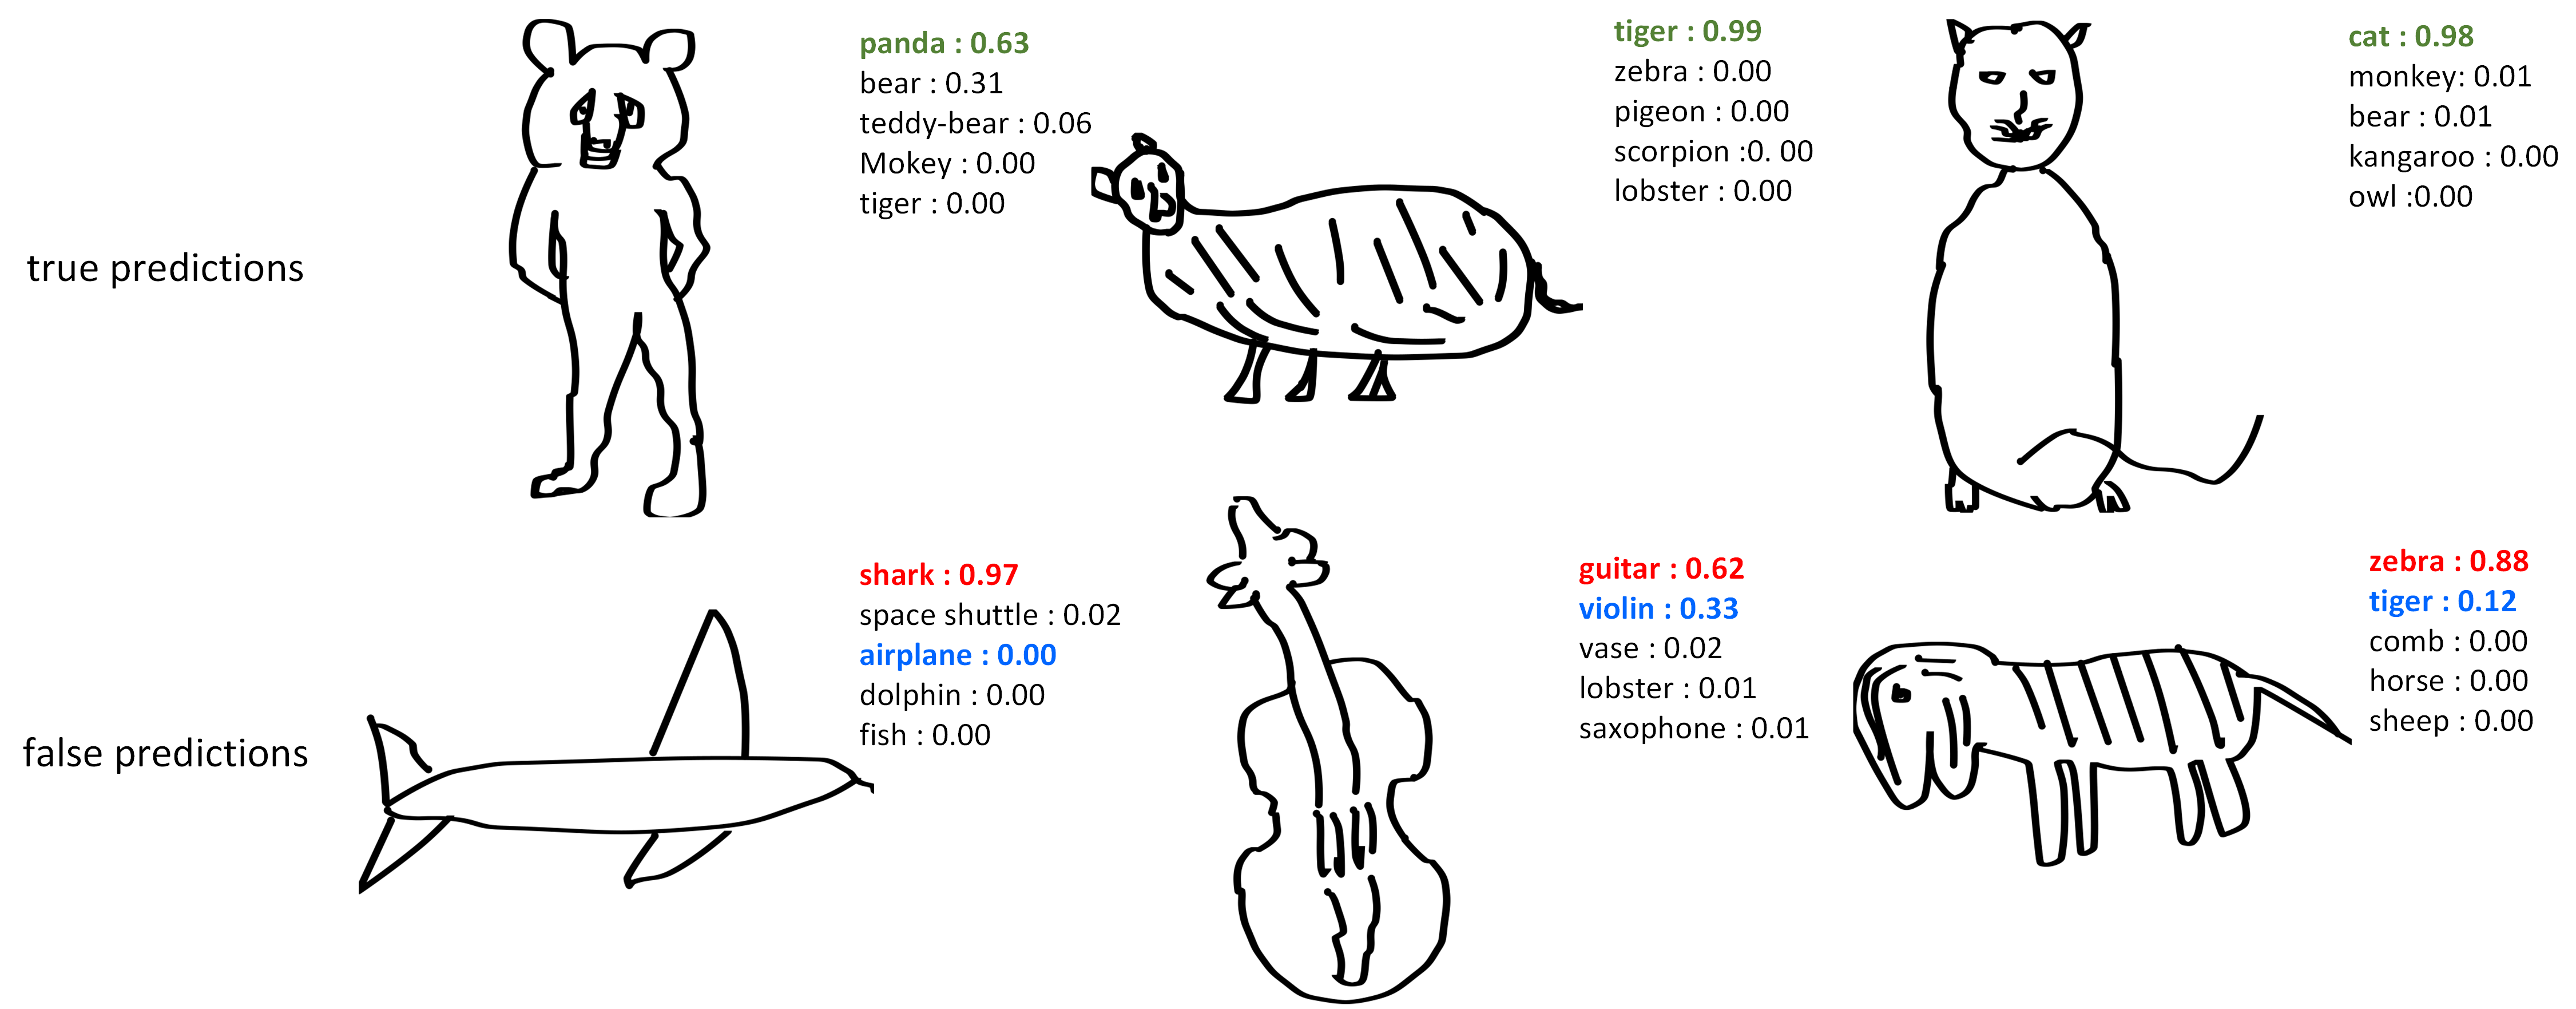
\includegraphics[width=3in]{images/res.png}
    \fcaption{Illustration of recognition successes (green) and failures (red).}
    \label{fig:resshow}
\end{figure}
